\documentclass{beamer}

\author{Chiel Kooijman\\5743028\\\url{Chiel999@gmail.com} \and
Steven Laan\\6036031\\\url{S.Laan@uva.nl} \and
Camiel Verschoor\\10017321\\\url{Verschoor@uva.nl} \and
Auke Wiggers\\6036163\\\url{A.J.Wiggers@uva.nl}}

\title{Visual SLAM\\ \normalsize Visual Odometry and SLAM with humanoid
robots.\\Project AI\\Artificial Intelligence\\Faculty of Science\\ University
of Amsterdam}

\usepackage{graphicx}

\begin{document}

\begin{frame}
	\begin{center}
		{\LARGE NAVIGATE}
	\end{center}

	\begin{center}
		\textsc{Nao Visual Gait And Trajectory Estimation:}\\
		\textsc{\small Monocular Visual Odometry on the Nao}
	\end{center}

	\begin{center}
		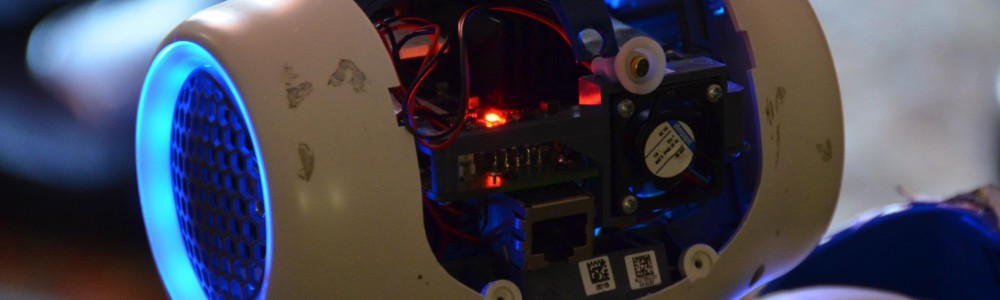
\includegraphics[scale=.3]{images/nao-head}
	\end{center}

	\begin{center}
		Chiel Kooijman, Steven Laan, Camiel Verschoor \& Auke Wiggers
	\end{center}
\end{frame}

\begin{frame}{Why Odometry?}
	\begin{quote}
		Odometry is the use of data from moving sensors to estimate change in
		position over time.
	\end{quote}

	\begin{itemize}
		\item Freely-moving agents need to know where they are to execute plan
		\item Movement in the real world is always subject to errors
	\end{itemize}
\end{frame}

\begin{frame}{Why Visual?}
	Alternatives:
	\begin{itemize}
		\item Sonar
		\item Laser range scanner
		\item GPS
	\end{itemize}

	Cameras:
	\begin{itemize}
		\item Are cheap, abundant, light, passive sensors
		\item	Work indoors
	\end{itemize}
\end{frame}

\begin{frame}{Using Camera Input for Odometry}
	\begin{itemize}
		\item Construct 3D representation from 2D images to determine camera
			position
		\item Needs to be fast enough for real-time computation
	\end{itemize}
\end{frame}

\begin{frame}{Calibration}
	Camera input is distorted (i.e. lines are not straight in corners)

	% TODO chessboard image
\end{frame}

\begin{frame}{Calibration}
	Use `chessboard' of known size:
	\begin{itemize}
		\item Find distortion coefficients
		\item Find camera matrix (expresses focal length in pixels)
	\end{itemize}

	% TODO distorted/undistorted image here
\end{frame}

\begin{frame}{Descriptors}
	To reconstruct 3D world we need to match points between images
	\begin{enumerate}
		\item Find salient points
		\item Make descriptor of points (using BRISK features: fast and robust)
		\item Match points, discard unlikely matches (with RANSAC)
	\end{enumerate}
\end{frame}

\begin{frame}{Homography}
	find positions of 2D points in 3D
	Images need to be sufficiently different for homography
	need keyframe selection to guarantee reliable reconstruction:
	* (mean shift - total shift):
	  near 0 indicates rotation of camera: does not contain 3D information
\end{frame}

\begin{frame}{Scale Ambiguity}
	
\end{frame}

\begin{frame}
	Initialize:
	\begin{enumerate}
		\item Calibrate (or use previous calibration parameters)
		\item Create initial 3D points from 2 images (world coordinates)
		\item Set camera position to $\vec{0}$
			\newcounter{enumTemp}
			\setcounter{enumTemp}{\theenumi}
	\end{enumerate}
	Loop:
	\begin{enumerate}
			 \setcounter{enumi}{\theenumTemp}
		\item Create new 3D points (image-to-image)
		\item Find position of camera relative to world coordinates (PnP)
		\item Find scale of new relative to world
		\item Translate \& scale new points to world
		\item Add to world coordinates
	\end{enumerate}
\end{frame}


% homography & keyframe selection
% egomotion
% 8-point algorithm?
% reconstruction & scale
% image-to-image
% image-to-world


\bibliographystyle{plainnat}
\bibliography{../report/references}

\end{document}
% vim: set spell : spelllang=en_gb :
